\documentclass[11pt]{amsart}
\usepackage[
style=authoryear, natbib=true,
]{biblatex}
\addbibresource{biblio.bib} 
%prepared in AMSLaTeX, under LaTeX2e
\addtolength{\oddsidemargin}{-.75in} 
\addtolength{\evensidemargin}{-.75in}
\addtolength{\topmargin}{-.6in}
\addtolength{\textwidth}{1.4in}
\addtolength{\textheight}{1.3in}
\renewcommand{\baselinestretch}{1.06}

\usepackage{wrapfig,fancyvrb,xspace}
\usepackage{palatino,bm}
\usepackage[final]{graphicx}
\usepackage[pdftex, colorlinks=true, plainpages=false, linkcolor=blue, citecolor=red, urlcolor=blue]{hyperref}

% macros
\newcommand{\bn}{\mathbf{n}}
\newcommand{\bq}{\mathbf{q}}
\newcommand{\bu}{\mathbf{u}}
\newcommand{\bw}{\mathbf{w}}
\newcommand{\bx}{\mathbf{x}}

\newcommand{\bX}{\mathbf{X}}

\newcommand{\bsigma}{\bm{\sigma}}
\newcommand{\bomega}{\bm{\omega}}

\newcommand{\cH}{\mathcal{H}}
\newcommand{\cK}{\mathcal{K}}
\newcommand{\cV}{\mathcal{V}}

\newcommand{\dx}{\mathrm{dx}}
\newcommand{\ds}{\mathrm{ds}}

\newcommand{\RR}{\mathbb{R}}

\newcommand{\Div}{\nabla\cdot}
\newcommand{\eps}{\epsilon}
\newcommand{\grad}{\nabla}
\newcommand{\lam}{\lambda}



\title{Gas in a porous media, using Firedrake}
\author{Tara Shreve}
\author{Ed Bueler}
\date{\today}

\begin{document}
\maketitle
%\begin{abstract}
%FIXME
%\end{abstract}

\thispagestyle{empty}

\section{A (draft) porous medium model for Darcy-type gas flow}

Suppose $\Omega$ is a 2-dimensional domain with well-behaved boundary, such as a rectangle or other polygon.  We will use $x$ for the horizontal and $z$ for the vertical coordinate.  We assume $z$ is measured positive upward.  Within $\Omega$ we assume there is a matrix of porous material with variable properties of porosity $\phi(x,z)$ and permeability $k(x,z)$; these are assumed independent of time.

Suppose that an ideal gas flows through that medium.  We will take various properties of the gas to be positive constants: $\mu$ is the dynamic viscosity, $R$ is the gas constant, $T$ is the absolute temperature, and $M$ is the molar mass.  The ideal gas law says $RT \rho = M P$.  The following system of equations, a mathematical model, applies to determing the evolution of the density $\rho(t,x,z)$, pressure $P(t,x,z)$, and vector volumetric flux $\bq(t,x,z)$:\footnote{TS: Please check that this is the model you want?}
\begin{subequations}
\label{eq:pmtime}
\begin{align}
\phi \frac{\partial \rho}{\partial t} + \Div \left(\rho\, \bq\right) &= 0 \label{eq:pmtime:masscont} \\
\bq &= - \frac{k}{\mu} \grad\left(c \rho + \rho g z\right) \label{eq:pmtime:darcy}
\end{align}
\end{subequations}
Here $c = RT/M$ is constant.  To be physical the density must be non-negative: $\rho\ge 0$.  In \eqref{eq:pmtime:masscont} we are assuming no mass sources or sinks in \eqref{eq:pmtime:masscont}, otherwise there could be a function on the right.  From the (litho)static pressure $P_0=-\rho g z$ note that $c\rho+\rho g z = P-P_0$, so we see that the flow in \eqref{eq:pmtime:darcy} is driven by deviations from static pressure.  The volumetric flux $\bq$ is related to the vector velocity $\bu$ by $\bq = \phi \bu$; the velocity $\bu$ may be helpful in diagnosing the solution but it is not needed to state the above.

It is straightforward to eliminate $\bq$ if desired:
\begin{equation}
\phi \frac{\partial \rho}{\partial t} - \Div \left(\frac{k}{\mu} \rho \grad\left(c \rho + \rho g z\right)\right) = 0.  \qquad \text{\emph{(porous medium equation)}} \label{eq:pmtime:primal}
\end{equation}
This form is comparable to the better-known heat equation
\begin{equation}
\frac{\partial u}{\partial t} - \Div(\grad u) = 0. \qquad \text{\emph{(heat equation)}}\label{eq:heattime:primal}
\end{equation}
An important property of \eqref{eq:heattime:primal} is that the operator $\Div \grad = \grad^2$ acts as a kind of invertible matrix, which assists in finding the solution $u$.  Since $\rho$ appears as a flux coefficient in \eqref{eq:pmtime:primal}, this invertibility will be lost if $\rho\to 0$ somewhere.  This ``degeneration'' of the diffusivity is a well-known property of the porous medium equation which may influence the numerical solution method.

System \eqref{eq:pmtime} is time dependent.  Its steady-state form is found by setting $\partial \rho/\partial t = 0$.  Also, to emphasize that mass is conserved we define the mass flux
	$$\bsigma = \rho \bq.$$
Thus the strong form for the steady-state problem can be written in terms of the conserved density $\rho$ and its flux $\bsigma$:
\begin{subequations}
\label{eq:pm:strong}
\begin{align}
\bsigma &= - \frac{k}{\mu} \rho \grad\left(c \rho + \rho g z\right) \label{eq:darcy} \\
\Div \bsigma &= 0 \label{eq:masscont}
\end{align}
\end{subequations}

\section{Weak form and finite element solution}

We will solve system \eqref{eq:pm:strong} by a conservative mixed finite element method \citep{Boffi2013} in which the flux $\bsigma$ is continuous across faces (edges) of the elements.  To derive the weak form we multiply \eqref{eq:darcy} by a vector-valued test function $\bomega$, and multiply \eqref{eq:masscont} by a scalar test function $v$, and integrate over $\Omega$:
\begin{subequations}
\label{eq:pm:prelim}
\begin{align}
\int_\Omega \bsigma\cdot \bomega\,\dx + \int_\Omega \frac{k}{\mu} \rho \grad\left(c \rho + \rho g z\right) \cdot \bomega\,\dx &= 0 \\
\int_\Omega (\Div \bsigma) v\,\dx &= 0
\end{align}
\end{subequations}
Here $\dx = dx\,dz$ denotes the area element.

Integration by parts will now use the divergence theorem
    $$\int_\Omega \Div \bX\,\dx = \int_{\partial\Omega} \bX\cdot \bn\,\ds$$
to remove the derivatives from the pressure $P=c\rho+\rho g z$.  Here $\ds$ denotes the integral over $\partial\Omega$ and $\bn$ denotes the outward normal unit vector on $\partial\Omega$.  We get the weak form
\begin{subequations}
\label{eq:pm:weak:early}
\begin{align}
\int_\Omega \bsigma\cdot \bomega\,\dx - \int_\Omega \frac{1}{\mu} \left(c \rho + \rho g z\right) \Div(k\rho\bomega)\,\dx + \int_{\partial\Omega} \frac{k}{\mu} \rho \left(c \rho + \rho g z\right) \bomega\cdot\bn\,\ds &= 0 \label{eq:pm:weak:early:darcy}\\
\int_\Omega (\Div \bsigma) v\,\dx &= 0
\end{align}
\end{subequations}
Notice that $k$ now appears inside a divergence in the first equation.

% FIXME: k and rho are discontinuous (and spatial varying) fields, so it is bad that they are inside the divergence

In order to write a final weak form, suitable for a Firedrake \citep{Ham2023}, we must choose suitable boundary conditions.  Along the part of the boundary $\partial\Omega$ where the pressure (or density) is determined, which we denote $\Gamma_0 \subset \partial\Omega$, the boundary integral in \eqref{eq:pm:weak:early:darcy} becomes a known linear functional on the test function $\bomega$.  The known value of the density in these location is denoted $\rho_0$.  On the remainder of the boundary we must impose the essential requirement that $\bomega\cdot \bn=0$ on the function space; this is done through Firedrake's \verb|DirichletBC()| command.  The resulting final weak form can be written as follows, with the known pressure boundary condition on the right:
\begin{subequations}
\label{eq:pm:weak}
\begin{align}
\int_\Omega \bsigma\cdot \bomega\,\dx - \int_\Omega \frac{1}{\mu} \left(c \rho + \rho g z\right) \Div(k\rho\bomega)\,\dx &= -\int_{\Gamma_0} \frac{k}{\mu} \rho_0 \left(c \rho_0 + \rho_0 g z\right) \bomega\cdot\bn\,\ds \label{eq:pm:weak:darcy}\\
\int_\Omega (\Div \bsigma) v\,\dx &= 0
\end{align}
\end{subequations}
The first equation in this system weakly enforces Darcy's law and the second enforces conservation of mass.

To implement the above in Firedrake we must choose finite element spaces for $\bsigma$ and $\rho$.  To provide exact discrete mass conservation the vector fields $\bsigma$ should come from a space in which normal vectors are continuous across element boundaries.  The space for $\rho$ can be discontinuous.  Thus, for example, we may use the lowest-order Raviart-Thomas and DG pair, over quadrilateral elements, which is stable for the mixed Poisson formulation:
\begin{Verbatim}[fontsize=\small,frame=lines]
S = FunctionSpace(mesh, 'RTCF', 1)
H = FunctionSpace(mesh, 'DG', 0)
W = S * H
w = Function(W)
sigma, rho = split(w)
omega, v = TestFunctions(W)
\end{Verbatim}
Weak form \eqref{eq:pm:weak} then corresponds to the UFL code
\begin{Verbatim}[fontsize=\small,frame=lines]
F = dot(sigma, omega) * dx \
    - (1.0/mu) * (c * rho + rho * g * z) * div(k * rho * omega) * dx \
    + (1.0/mu) * k * rho0 * (c * rho0 + rho0 * g * z) * dot(omega, n) * ds(i) \
    + div(sigma) * v * dx
\end{Verbatim}
Here \verb|n = FacetNormal(mesh)|.  Note that \verb|ds(i)| requires indices \verb|i| for the appropriate boundary segments.

To solve the equations we apply Newton's method \citep{Kelley2003}.  Newton's method is managed by the SNES component of PETSc \citep{Balay2023}.  Some useful options are to use the default ``line search'' Newton solver \texttt{newtonls} but with the (non-default) back-tracking type of line search.  The linear Newton step equation are solved by a sparse direct matrix method \citep{Amestoy2001}.  Also we ask for feedback on the success or failure of the solver:
\begin{Verbatim}[fontsize=\small,frame=lines]
solve(F == 0, w, bcs=[BCs,],
      solver_parameters = {'snes_type': 'newtonls',
                           'snes_linesearch_type': 'bt',
                           'snes_rtol': 1.0e-5,
                           'snes_monitor': None,
                           'snes_converged_reason': None,
                           'ksp_type': 'preonly',
                           'pc_type': 'lu',
                           'pc_factor_mat_solver_type': 'mumps'})
\end{Verbatim}
A more advanced iterative, block-wise, and multigrid solver is possible \citep[e.g.][]{Bueler2021}, but it will require careful development.

Confirmation of global mass conservation is straightforward.  For example, on a rectangular domain with top side index \verb|4| and bottom side index \verb|3|:
\begin{Verbatim}[fontsize=\small,frame=lines]
topflux = assemble(dot(sigma,n) * ds(4))
bottomflux = assemble(dot(sigma,n) * ds(3))
imbalance = topflux + bottomflux
print(f'  flux out of top    = {topflux:13.6e}')
print(f'  flux into bottom   = {-bottomflux:13.6e}')
print(f'  imbalance          = {imbalance:13.6e}')
\end{Verbatim}
These \verb|assemble| expressions compute mass flux integrals
    $$\int_{\Gamma_i} \sigma\cdot \bn\,\ds = \int_{\Gamma_i} \rho \bq\cdot \bn\,\ds$$
over a particular side $\Gamma_i$.  In a typical run we get fluxes which balance to rounding error:
\begin{Verbatim}[fontsize=\small,frame=leftline]
  flux out of top    =  1.315019e+01
  flux into bottom   =  1.315019e+01
  imbalance          = -1.953993e-14
\end{Verbatim}


\section{An application for gas flow through a porous lava dome}

In \cite{Graham2023}, we measure permeability of samples from various textural units of the Obsidian dome and South Deadman dome using field and lab permeameters. These two domes are silicic lava flows in the Inyo Craters portion of the Mono-Inyo Craters in eastern California, a chain of silicic lava flows, domes, and explosion craters that stretches 12 km (7.5 miles) to the north-northeast of Long Valley Caldera. The Inyo craters erupted as recently as ~675 years (~1350 A.D.) before present. Prior studies subdivided the majority of the lava erupted at the Inyo Craters according to the observed vesicle textures found in different parts of each flow, subdivided into finely vesicular pumice (FV), coarsely vesicular pumice (CV), and dense obsidian (OB). Shallow scientific bore hole drilling in the 1970's confirmed the presence of an underground magmatic intrusion, which was the source of the domes. This drilling also provided some general constraints on the depth of each distinct textural unit within the dome (Table \ref{tab:UnitPermPoro}).

In this study, we wish to put constraints on the surface gas flux for each textural unit at Obsidian Dome. The unit mapping of the dome is shown in Fig. \ref{fig:unitMapping}, and an example cross-section is shown in Fig. \ref{fig:crossSection}. Using constraints on dome height, the depth and permeability of each unit, and assuming a significant portion of gas is sourced from degassing of the underlying feeder dike, we can use Darcy's law to calculate the surface gas flux through each unit. This was done in \cite{Graham2023} using a 1D model of Darcy's law, as implemented in \cite{Edmonds2003}, and we wish to extend this model into 2-dimensions, to account for the unit layering, which may affect the path of gas flow towards the surface.

COMSOL model results for gas density and surface gas flux are shown in Fig. \ref{fig:COMSOLresults}, with annotations stating relevant boundary conditions. Here we assume atmospheric pressure at the surface ($P_{atm} = 1.01325$ bar) and a pressure at the base of the dome ($L=22$ m) of $P_{z=L} = 11$ bar. There is a gas inlet at the base of the CV unit, through which steam at a temperature of 920$^{\circ}$C can enter the dome porous matrix. For simplicity, a no flow condition is imposed at the unit sides, and we choose to solve for the steady-state isothermal, compressible gas flow using Darcy's Law to relate volumetric gas flux and pressure. The porosity and permeability for each unit, as well as their height and percent of total dome surface area, are shown in Table \ref{tab:UnitPermPoro}.

\begin{figure}
   \centering
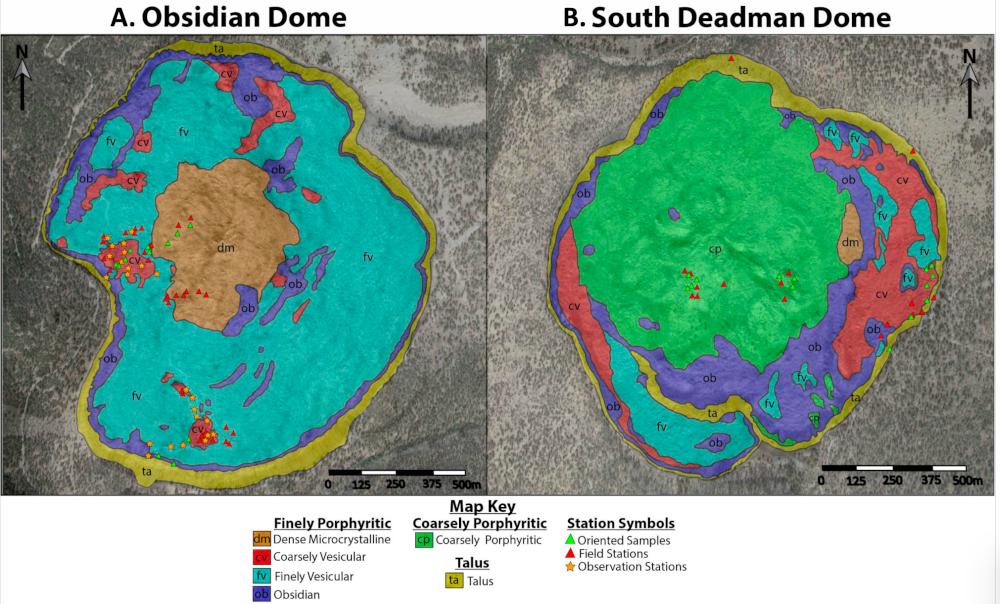
\includegraphics[width=0.95\textwidth]{figs/unitMapping-small.png}
\caption{Textural lithologic distribution maps of lavas for (A) Obsidian dome and (B) South Deadman dome.}
\label{fig:unitMapping}
\end{figure}

\begin{figure}
   \centering
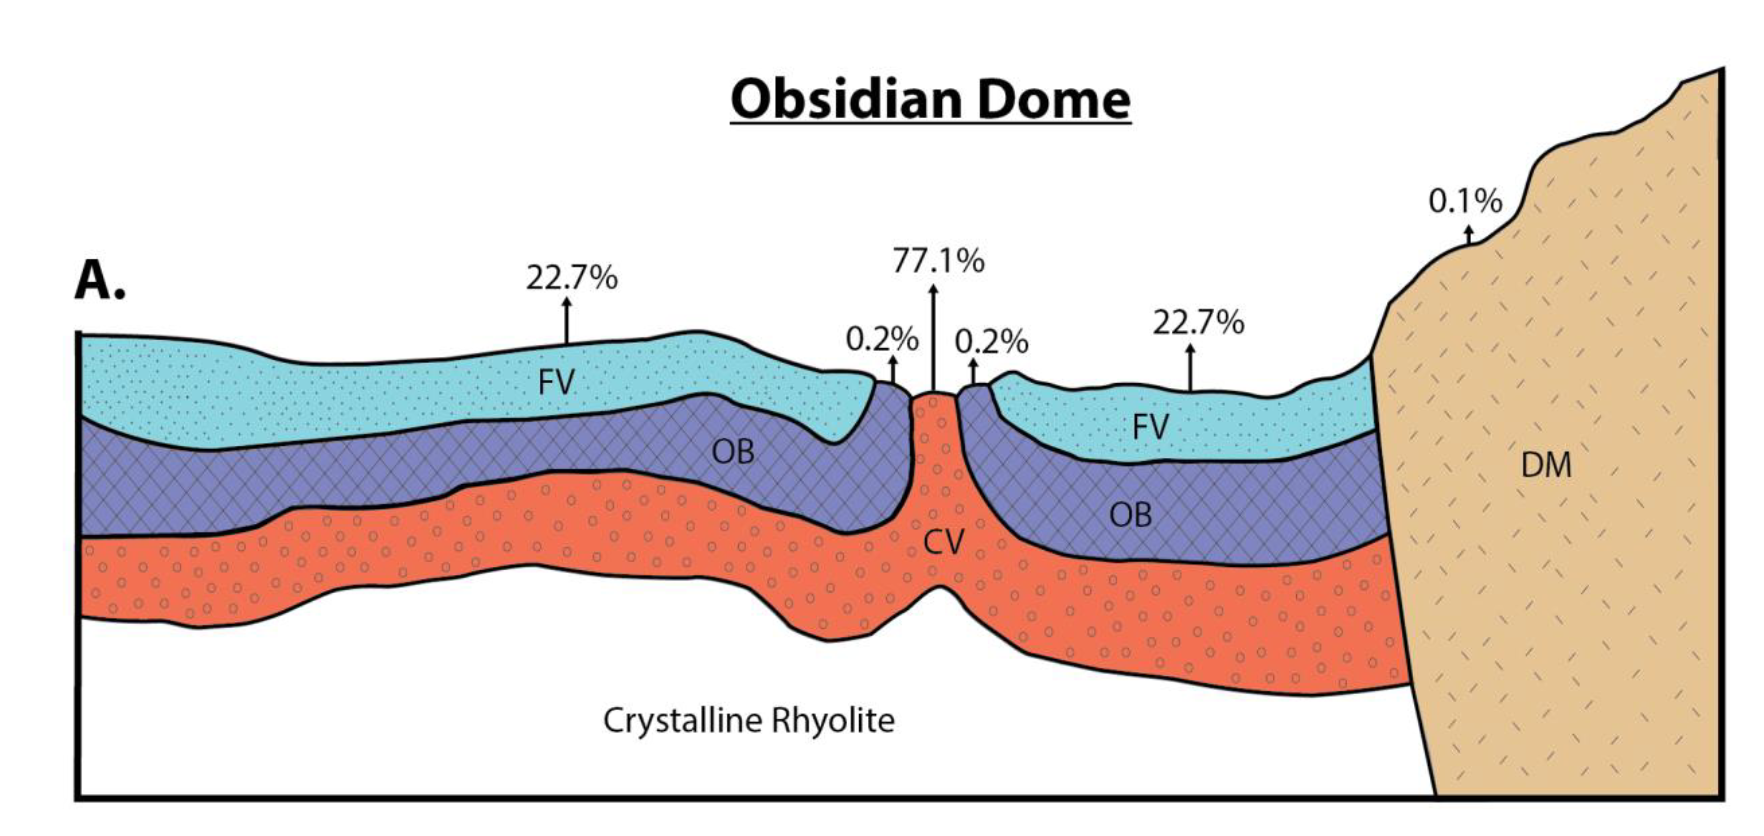
\includegraphics[scale=0.5]{figs/crossSection.png}
\caption{Schematic diagrams depicting total calculated gas flux percentages during the final stages of lava emplacement at Obsidian dome. Total gas flux for each lithologic unit was calculated using the gas flux model of Edmonds et al. (2003), and the gas flux percentages represent the percent gas flux for each lithologic unit relative to the total gas flux calculated for all units, and does not consider additional degassing that occurs through conduit processes, fractures, tuffisite veins, or porous pathways that are too large to measure.}
\label{fig:crossSection}
\end{figure}

\begin{figure}
   \centering
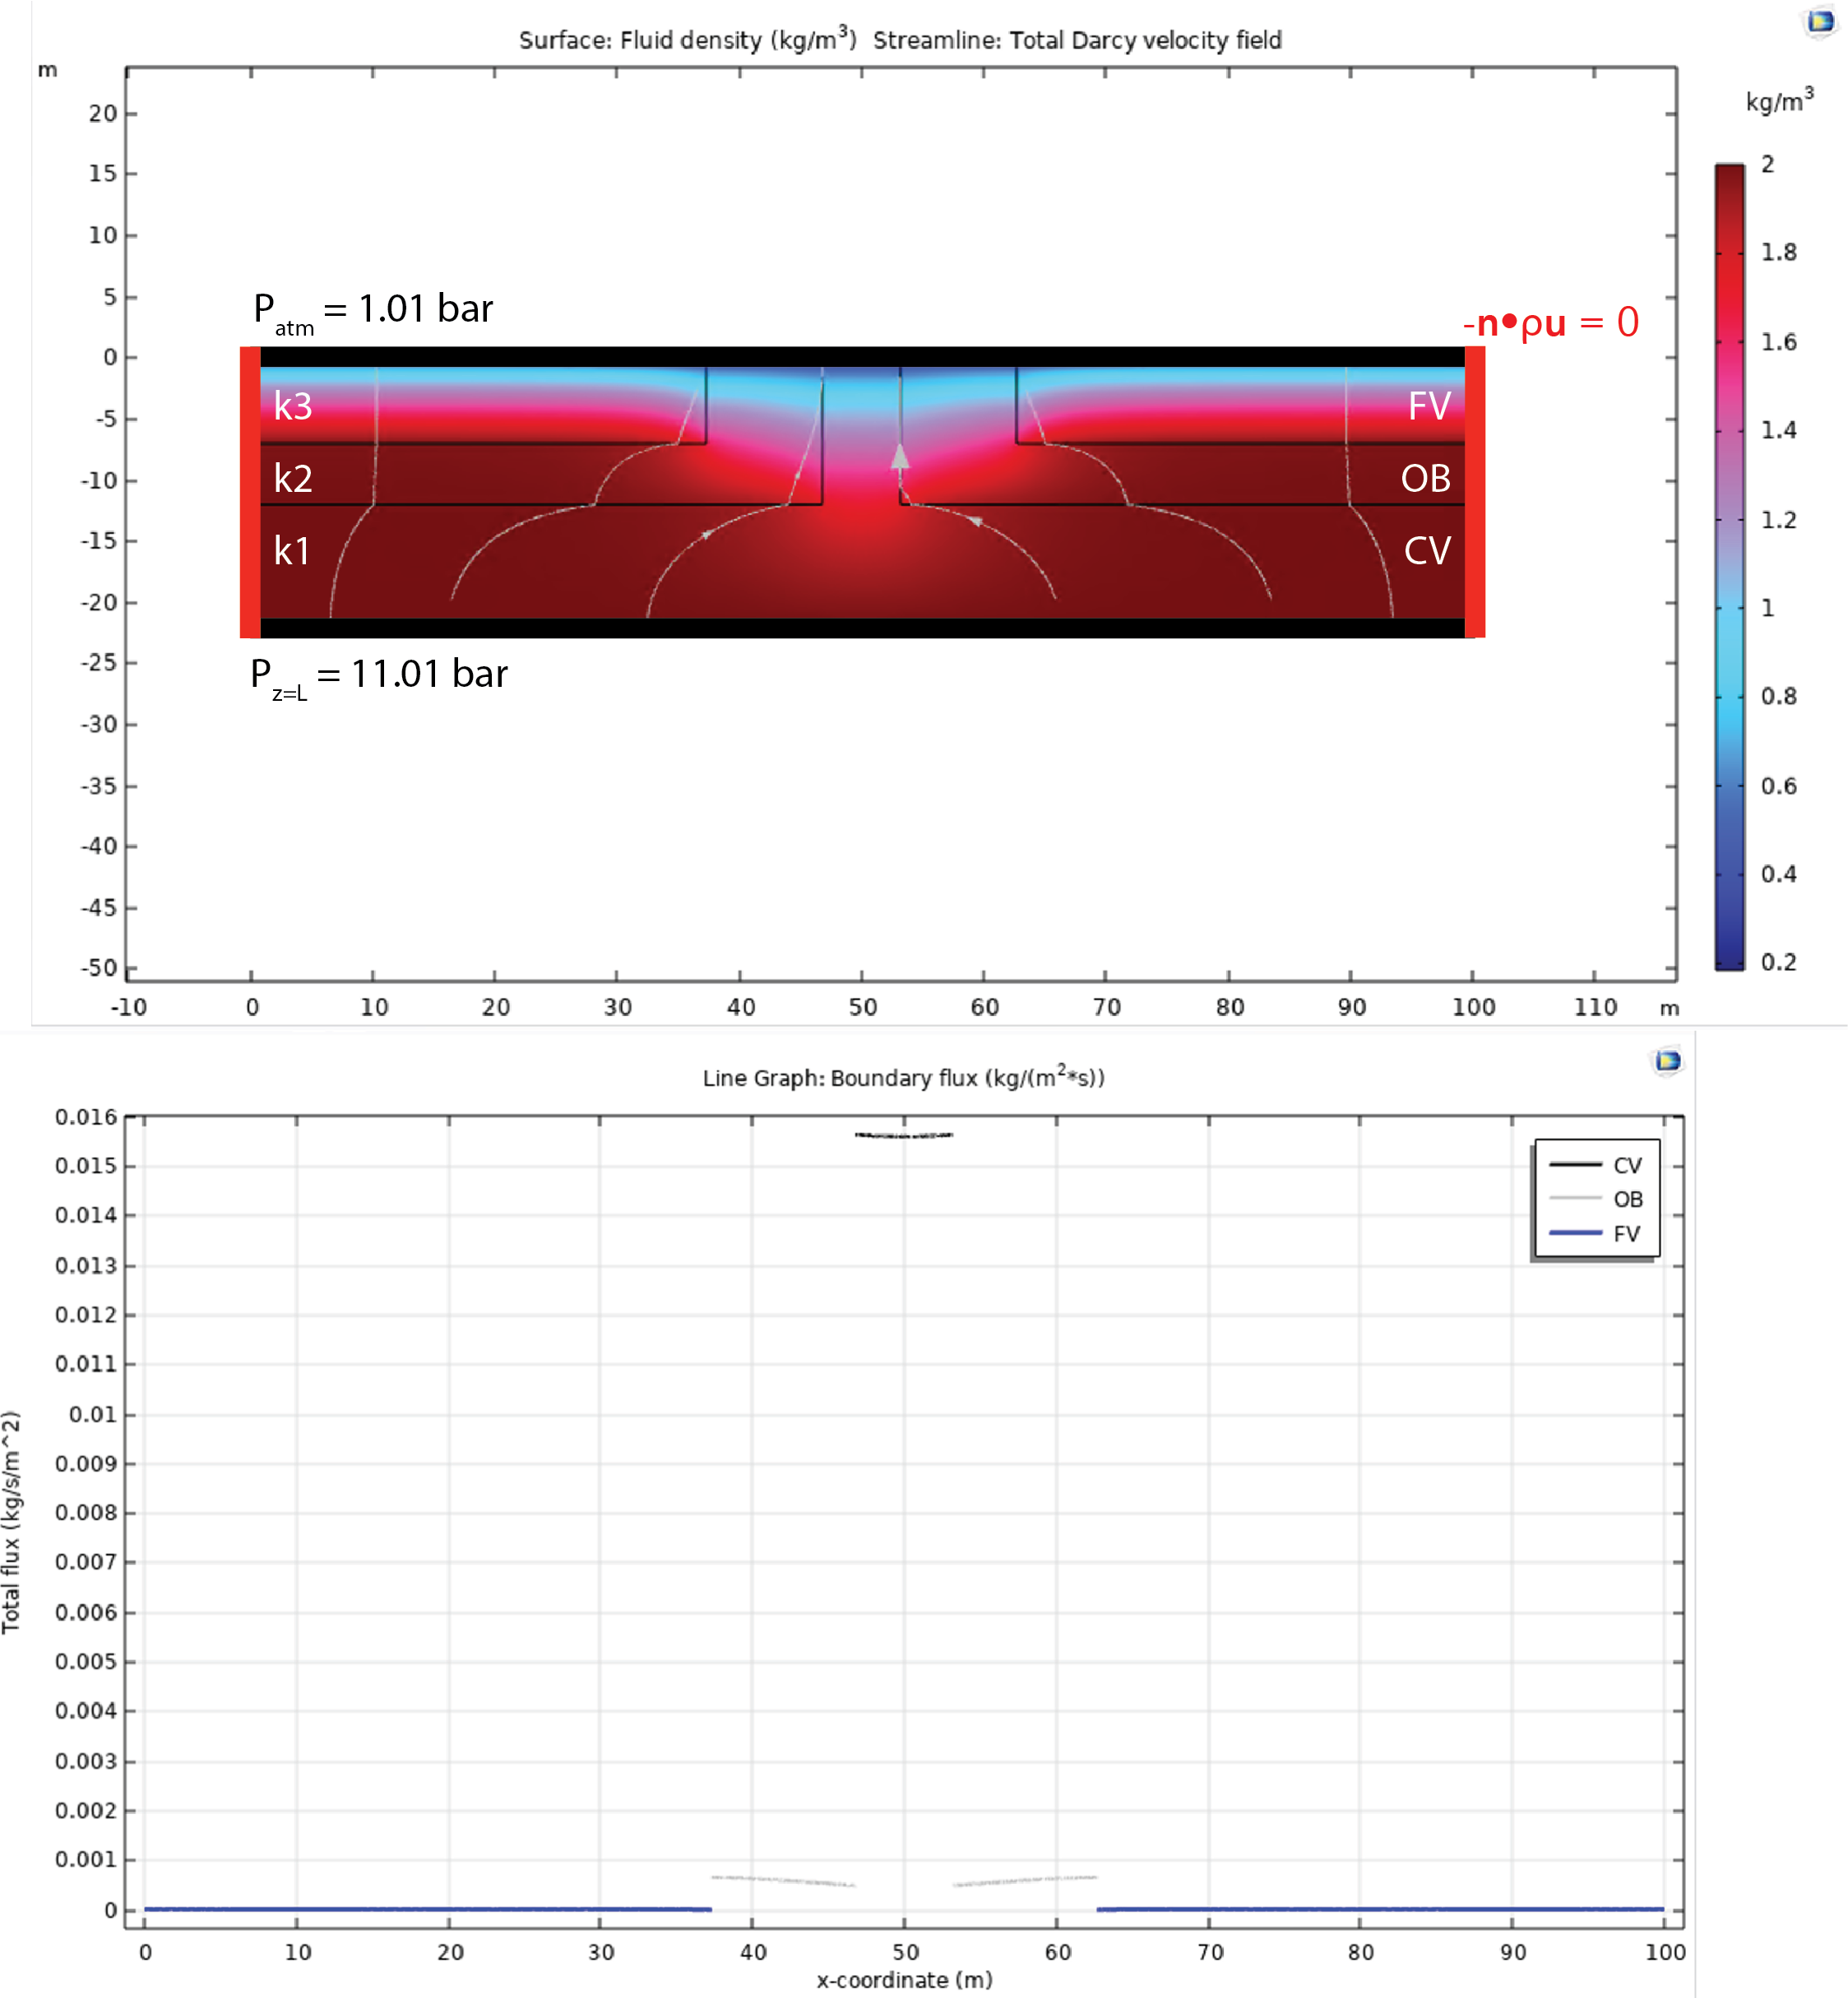
\includegraphics[scale=0.8]{figs/comsolDarcyLaw_units.png}
\caption{Top figure shows gas density in unit layers CV, FV, and OB, with permeabilities k1, k2, and k3, respectively (see Table \ref{tab:UnitPermPoro}). Streamlines indicate the direction of gas flow. Pressure boundary conditions at the base and surface of the units are shown in black, and no flow boundary conditions at the side of the units are shown in red. The bottom figure shows the gas flux at the surface.}
\label{fig:COMSOLresults}
\end{figure}


\begin{table}[h]
\center
      \small
      \begin{tabular}{lllll}
      \hline
      \textbf{Unit} & \textbf{Permeability (m\textsuperscript{2})} & \textbf{Connected porosity (\%)}  & \textbf{Height (m)} & \textbf{Percent of total dome surface area} \\  
      \hline
      CV & 6.87E-12 & 50.0 & 10 & 6.4 \\
      FV & 2.18E-13 & 23.2 &  7 & 74.6 \\
      OB & 4.94E-15 & 3.24 & 5 & 19.0 \\ 
\end{tabular}%}
\caption{Average permeability, porosity, height, and percent of total dome surface area of each textural unit.} 
\label{tab:UnitPermPoro}
\end{table}

\printbibliography

\end{document}
